\documentclass[a4paper,10pt,titlepage]{article}
  
\usepackage[utf8]{inputenc}
\usepackage[T1]{fontenc}
\usepackage[english]{babel}

\usepackage[usenames,dvipsnames]{color}
\usepackage{fancyhdr}
%\usepackage{lastpage}
\usepackage{float}
\usepackage{fancyvrb}

\usepackage{amssymb}
\usepackage{amsmath}
\usepackage{listings}
\usepackage{pdfpages}

\usepackage{graphicx}

\usepackage[parfill]{parskip}
\usepackage{textcomp}
\usepackage{lastpage}

\usepackage{tikz}
\usetikzlibrary{arrows,decorations.pathmorphing,backgrounds,positioning,fit,matrix}

\DeclareGraphicsExtensions{.png}


\definecolor{Viridian}{rgb}{0.25,0.51,0.43}
\definecolor{dkgreen}{rgb}{0,0.45,0}
\definecolor{gray}{rgb}{0.5,0.5,0.5}
\definecolor{mauve}{rgb}{0.30,0,0.30}


% keyword coloring for vitaly programs
\lstdefinelanguage{vitaly} {	
	morekeywords={func,end,var,type,int,bool,array,of,record,
		length,true,false,null,return,write,allocate,
		if,then,else,endif,while,do,for,
		system,break,continue,string
	},
	sensitive=true,
	morecomment=[l]{\#},
	morecomment=[s]{(*}{*)},
	morestring=[b]"
}

% Default settings for code listings
% Default settings for code listings
\lstset{frame=tb,
  %language=vitaly,
  aboveskip=3mm,
  belowskip=3mm,
  showstringspaces=false,
  columns=flexible,
  basicstyle={\small\ttfamily},
  numbers=left,
  numberstyle=\footnotesize,
  keywordstyle=\bfseries\color{Cerulean},
  commentstyle=\color{Viridian},
  stringstyle=\color{Fuchsia},
  frame=single,
  breaklines=true,
  breakatwhitespace=false,
  tabsize=4,
}

\fancypagestyle{compiler}{
\fancyhf{}
\fancyhead[L]{DM545}
\fancyhead[R]{\thepage /\pageref{LastPage}}
}

\title{DM545\\\rule{10cm}{0.5mm}\\Linear and Integer Programming}
\author{Jesper Lund\\jelun11@student.sdu.dk}
\begin{document}
\newcommand{\IS}{:}
\newcommand{\OR}{$|$}
\newcommand{\T}[1]{{\bf #1}}
\newcommand{\NT}[1]{$\langle$#1$\rangle$}


\begin{titlepage}
  \maketitle
\end{titlepage}

\pagestyle{compiler}

\tableofcontents
\newpage

\section{Examples}
\subsection{Network Flow}
\begin{figure}
\label{graph}
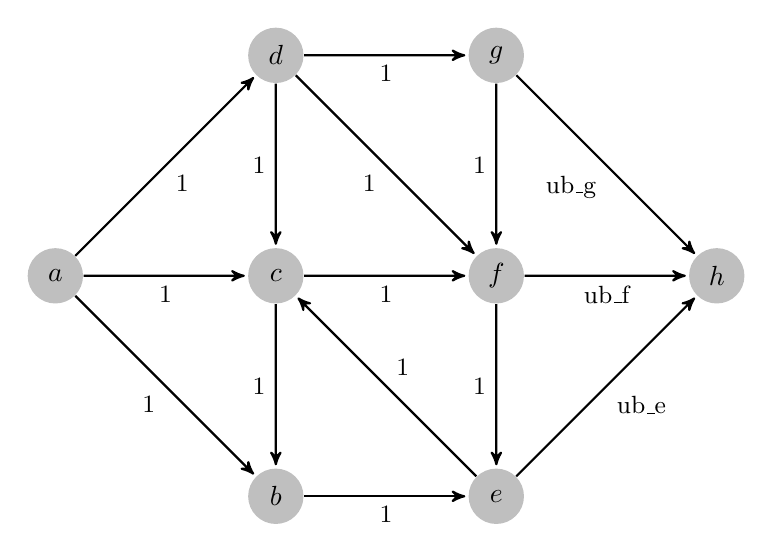
\begin{tikzpicture}[scale=1.4, auto,swap]
\tikzstyle{vertex}=[circle,fill=black!25,minimum size=20pt,inner sep=0pt]
\tikzstyle{selected vertex} = [vertex, fill=red!24]
\tikzstyle{edge} = [draw,thick,-]
\tikzstyle{arc} = [draw,thick,->,shorten >=1pt,>=stealth']
\tikzstyle{weight} = [font=\small]
\tikzstyle{selected edge} = [draw,line width=5pt,-,red!50]
\tikzstyle{ignored edge} = [draw,line width=5pt,-,black!20]

    % First we draw the vertices
    \foreach \pos/\name in {{(0,2)/a}, {(2,0)/b}, {(2,2)/c},
                            {(2,4)/d}, {(4,0)/e}, {(4,2)/f}, {(4,4)/g}, {(6,2)/h}}
    \node[vertex] (\name) at \pos {$\name$};
    % Connect vertices with edges and draw weights
    \foreach \source/ \dest /\weight in {
      a/b/1,
      a/c/1,
      a/d/1,
      d/c/1,
      c/b/1,
      d/g/1,
      d/f/1,
      c/f/1,
      b/e/1,
      e/c/1,
      g/f/1,
      f/e/1,
      g/h/$ub\_g$,
      f/h/$ub\_f$,
      e/h/$ub\_e$}
      \path[arc] (\source) -- node[weight] {$\weight$} (\dest);

\end{tikzpicture}
\end{figure}

\subsection{Matrices}
\begin{table}[h]
\centering
\caption{Eksempel}
\label{my-label}
\begin{tabular}{|l|l|l|l|l|l|l|l|l|l|}
\hline
$x_1$ & $x_2$ & $x_3$ & $x_4$ & $x_5$ & $x_6$ & $x_7$ & $x_8$ & z & b \\ \hline
     &      &      &      &      &      &      &  &   &   \\ \hline
     &      &      &      &      &      &      &  &   &   \\ \hline
     &      &      &      &      &      &      &  &   &   \\ \hline
\end{tabular}
\end{table}
\subsection{Cut example}
\begin{center}
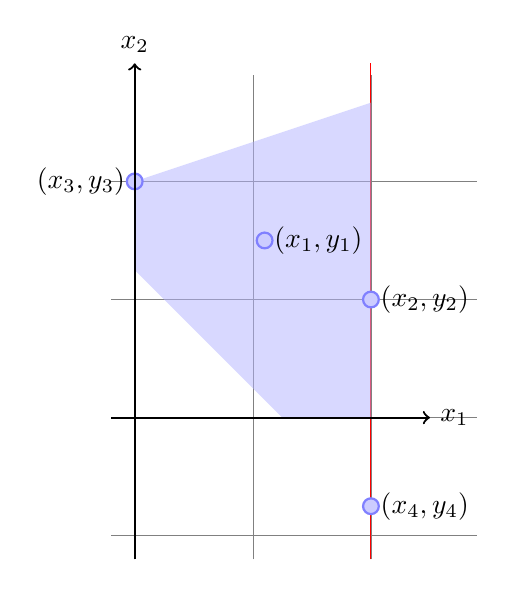
\begin{tikzpicture}[domain=-0.1:2.2,xscale=1.5,yscale=1.5,
basis/.style={circle,draw=blue!50,fill=blue!20,thick,inner sep=0pt,minimum size=2mm},
opt/.style={circle,draw=red!50,fill=red!50,thick,inner sep=0pt,minimum size=2mm},
point/.style={rectangle,draw=black!50,fill=black!20,thick,inner sep=0pt,minimum size=4mm}]

\draw[very thin,color=gray] (-0.2,-1.2) grid (2.9,2.9);
\draw[color=red] plot[id=c0]  function{2 +0.33*x} node[right] {};

\draw[color=red] (2,-1.2) -- (2,3) node[right] {};

\draw[color=red] plot[id=c2, domain=-0.1:2.3]  function{1.2500 -x} node[right] {};

\fill[blue!30,opacity=0.5]
(2,2.666667) -- %
(0,2) -- %
(0,1.25) -- %   
(1.25,0) -- %    
(2,0);


\node (p1) at (1.1,1.5) [basis] {};
\node at (p1) [right] {($x_1,y_1$)};
\node (p2) at (2,1) [basis] {};
\node at (p2) [right] {($x_2,y_2$)};
\node (p3) at (0,2) [basis] {};
\node at (p3) [left] {($x_3,y_3$)};
\node (p4) at (2,-3/4) [basis] {};
\node at (p4) [right] {($x_4,y_4$)};

\draw[->,thick] (-0.2,0) -- (2.500000,0) node[right] {$x_1$};
\draw[->,thick] (0,-1.2) -- (0,3) node[above] {$x_2$};
\end{tikzpicture}
\end{center}
\subsection{Java Simplex}
(1) gå til src og ``javac JavaSimplex.java''\\
(2) brug java simplex med ``java JavaSimplex \%inputfile\%''\\
(3) f.eks. ``java JavaSimplex exam.eqn''
\end{document}
